\documentclass[letterpaper,11pt]{article}

\usepackage[empty]{fullpage}
\usepackage[x11names]{xcolor}
\usepackage[utf8]{inputenc}
\usepackage[frenchb]{babel}
\usepackage{graphicx}
\usepackage[colorlinks=true, urlcolor=RoyalBlue4, pdftitle={CV Quentin Casasnovas}, pdfauthor={Quentin Casasnovas}, pdfsubject={CV Quentin Casasnovas}]{hyperref}

\raggedbottom
\raggedright
\setlength{\tabcolsep}{0in}

\addtolength{\oddsidemargin}{-0.5in}
\addtolength{\evensidemargin}{-0.5in}
\addtolength{\textwidth}{1.0in}
\addtolength{\topmargin}{-0.5in}
\addtolength{\textheight}{1.0in}

\hypersetup{
  pdfborder=0 0 0}


% Custom commands

\newcommand{\resitem}[1]{\item #1}

\newcommand{\titlecolor}[0]{RoyalBlue4}
\newcommand{\bulletcolor}[0]{darkgray}

\newcommand{\resheading}[1]{
  \vspace{10pt}
  {\Large
        \textsc{\textcolor{\titlecolor}{\textbf{#1}}}
  } \\
  \vspace{-10.5pt}
  \hspace{-1pt}\textcolor{\titlecolor}{\line(1,0){525}}
}

\newcommand{\ressubheading}[4]{
  \vspace{8pt}
  \begin{tabular*}{7.0in}{l@{\extracolsep{\fill}}r}
    \textsc{#1} & #2 \\
    \textsl{#3} & \textit{#4} \\
  \end{tabular*}
}

\newcommand{\prettylist}[0]{
  \begin{itemize}
    \renewcommand{\labelitemi}{{\tiny \textcolor{\bulletcolor}{$\bullet$}}}
    \renewcommand{\labelitemiii}{$\cdot$}
}

\newcommand{\projectlist}[0]{
  \begin{tabular}{p{0.03\linewidth}p{0.4\linewidth}p{0.1\linewidth}p{0.4\linewidth}}
    & \begin{itemize}
}

\newcommand{\projectitem}[1]{
  \vspace{3pt}
  \item[ \textcolor{\bulletcolor}{{\tiny $\bullet$}} {\small \textsc{#1}}]
}

\newcommand{\projectsep}[0]{
      \end{itemize} & & \begin{itemize}
}

\newcommand{\projectlistend}[0]{
\end{itemize}
\end{tabular}
}

\newcommand{\acro}[1]{
  {\small\textsc{#1}}\hspace{-3pt}
}

% Document


\begin{document}

\begin{minipage}{0.40\linewidth}
{\LARGE \textbf{\textcolor{\titlecolor}{Quentin Casasnovas}}}\\
\vspace{2pt}
\begin{tabular}{p{0.007\linewidth}l}
 & {\small \textcolor{\titlecolor}{920 TOEIC}} \\
 & {\small \textcolor{\bulletcolor}{\url{http://uk.linkedin.com/in/quentincasasnovas}}} \\
 & {\small \textcolor{\bulletcolor}{French nationality, 25 years old}} \\
 & {\small \textcolor{\bulletcolor}{quentin.casasnovas@gmail.com}} \\
 & {\small \textcolor{\bulletcolor}{39 \acro{Steamship House} - \acro{Gas Ferry Road}}} \\
 & {\small \textcolor{\bulletcolor}{BS1 6GL \acro{Bristol - England}}} \\
 & {\small \textcolor{\bulletcolor}{+44 7743 389 757}} \\
\end{tabular}
\end{minipage}
\begin{minipage}{0.54\linewidth}
\begin{flushright}
%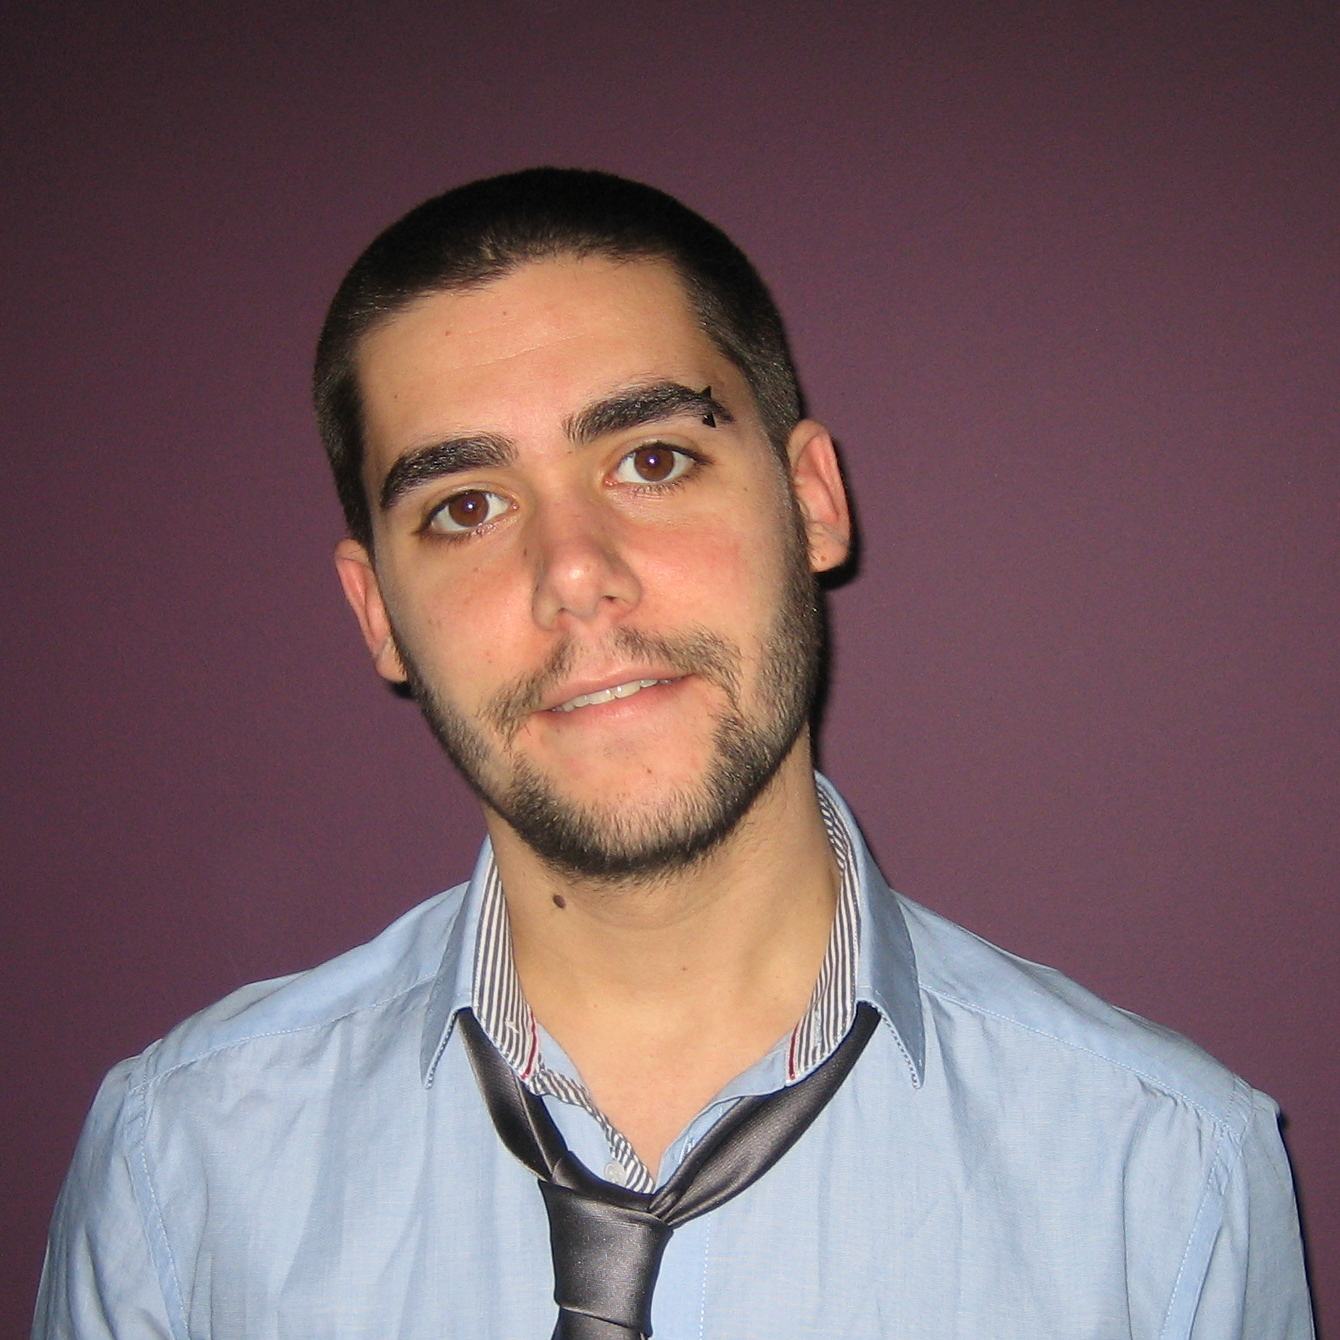
\includegraphics[scale=0.07]{id.png}
\end{flushright}
\end{minipage}

\vspace{8pt}
\resheading{Goals}
\begin{minipage}{0.95\linewidth}
\vspace{10pt}
\paragraph{}
My main area of interest is kernel development, shall it be low level kernel
development such as device driver implementation, or at a higher level with
userland interaction. I'm thrived by challenging projects involving
complex interactions between the hardware all the way through to userland.
\paragraph{}
I'm especially attracted by companies which work with/on open source project
like the Linux kernel, and which have a strong technical/innovation
background. A company putting a lot of effort in R\&D is a plus, so as one
using agile software development methods and valorisating technical
expertise.

\end{minipage}

\resheading{Experience}
\prettylist
\item
  \ressubheading{MathEmbedded, Permanent Contract}{Bristol, England}{Embedded Engineer - Tech Lead}{Dec. 2010 - today}
  \begin{itemize}
    \resitem{Split of grsecurity patch by features, implementation of regression tests for grsecurity}
    \resitem{Boot time optimizations for different STBs running STLinux}
    \resitem{Conception \& implementation of an automated remote tracing mechanism to certify the security of STBs}
    \resitem{Requirements capture on customer's site}
    \resitem{Support and documentation for the customer}
  \end{itemize}
\item
  \ressubheading{Scaleo Chip, Final Internship}{Sophia Antipolis, Alpes Maritimes}{Reducing power consumption on \acro{Linux-SMP SoC}}{Feb. 2010 - Sep. 2010}
  \begin{itemize}
    \resitem{Implementation of cpu hotplug/hotunplug for sparc architectures on
      \acro{Linux}} 
      \resitem{Dynamically stop/start back CPU depending on system load}
    \resitem{Development of Python/Qt UI to monitor the current consumption
      of the platform}
  \end{itemize}
\item
  \ressubheading{DCNS, Internship}{Toulon, Var}{Improvement of the HMI of a sub-marine simulator}{Jun. 2008 - Aug. 2008}
  \begin{itemize}
    \resitem Development in\acro{OpenMotif/C}
  \end{itemize}
\item
  \ressubheading{McDonald's Grand Ciel, Permanent contract}{La Garde,
    Var}{Teammate then team leader}{Sep. 2004 - Apr. 2008}
  \begin{itemize}
    \resitem Manager responsible for training and supplies the last two years
  \end{itemize}
\end{itemize}

\resheading{Education}
\prettylist
\item
  \ressubheading{EPITA}{Paris XIII, Île de France}{Engineering degree -
    Embedded and Real Time systems}{Sep. 2008 - Sep. 2010}
  \begin{itemize}
    \resitem{Member of the research laboratory LSE (Laboratoire Systèmes
      d'Exploitation)}
  \end{itemize}
\item
  \ressubheading{USTV}{La Garde, Var}{Bachelor's degree in Systems
    Informationnal Security}{Sep. 2004 - Apr. 2008}
  \begin{itemize}
    \resitem{Tutoring of 1\textsuperscript{st} year students}
  \end{itemize}
\item
  \ressubheading{High School Jean Aicard}{Hyères, Var}{Scientific High School
    Graduation - Math option}{Sep. 2001 - Jul. 2004}
  \begin{itemize}
    \resitem{One semester in Toronto, Canada in complete immersion}
  \end{itemize}
\end{itemize}

\clearpage

\resheading{Skills}
\begin{description}
\item[Operating systems]
  Strong\acro{GNU/Linux;} Basics with {Android}
\item[Languages]
  \acro{Expert in C; Already worked with C++, D, Python, Perl, Shell, Ada}
\item[Conception]
  \acro{Basics with Merise, UML}
\item[Things I use every day]
  \acro{git, emacs, ssh, bitlbee, gcc, gentoo, latex, gdb, toothbrush}
\end{description}
\vspace{-14pt}

\begin{tabular}{p{0.47\linewidth}p{0.05\linewidth}p{0.38\linewidth}}
\begin{description}
\item[Miscellaneous]
  {\small
    \begin{itemize}
    \item[ ]
    \item Fluent english speacker (920 TOEIC)
    \item Good problem solving skills
    \item Deliver secure, well documented code
    \item Web stuffs (SQL, php, javascript, ajax {\tiny\ldots} )
    \end{itemize}
  }
\end{description}
 & &
\begin{description}
\item[Human]
  {\small
    \begin{itemize}
    \item[ ]
    \item Excellent adaptability
    \item Autonomous
    \item Good communication skills
    \item Strong team spirit
    \end{itemize}
  }
\end{description}
\end{tabular}

\resheading{Relevants projects}
\projectlist


\vspace{3pt} \projectitem{Scalopes.} During my internship at Scaleo Chip, I had
the chance to work on the Linux kernel, notably for the leon3 sparc
processor. My objective was to reduce the power consumption of an embedded
platform in the context of the \href{http://www.scalopes.eu}{\acro{scalopes}} european project by implementing automatic clock gating in the Linux kernel. You can find a demo of my work on \href{http://www.dailymotion.com/video/xf6y9b_dynamic-hotplug-cpu-on-leon3_tech}{dailymotion} and the actual kernel module on \href{https://github.com/casasnovas/rm}{github}. As part of this project, I've also created an open source tool, \href{https://github.com/casasnovas/greth}{greth}, to interface the \acro{greth} open source hardware block from \acro{Gaisler.}

\vspace{3pt} \projectitem{Remote tracing.} Designed and implemented a remote
tracing mechanism using the Linux kernel kprobes API to automate the security
certification process of STBs for a known CA vendor. The system supports arm,
mips, sh and x86 and can be driven remotely by a web UI. I've also participated
in the customer's requirements capture on site.

\projectsep

\projectitem{Amee} is a robotic project developped as part of my last year
study. The principle is to use a FreeRunner cellphone (ARM420) as the robot
brain, connecting it to a \acro{usb} board with an embedded AVR microchip,
itself connected to various other parts of the robot (telemeter, CC motors,
{\tiny\ldots}). The big interest lies in the huge number of sensors offered
nativly by the phone (\acro{gps}, accelerometer, {\tiny\ldots}) and its
connecting interface (\acro{wifi}, bluetooth, \acro{usb}, {\tiny\ldots}). You
can find more about this at \url{http://gistr.epita.fr} in the project area.

\vspace{3pt} \projectitem{Multitouch driver.} As part of my last year study, I
integrated a multitouch capable panel to the FreeRunner cellphone. I developed
a Linux driver which supports \acro{Lumio USB} multitouch panel. I was in close
collaboration with \acro{Lumio} software team, which invited me for a week in
Israel to train them on the Linux driver, and extend the driver to their new
firmware. You can find the source code and documentation of this driver on my
\href{http://github.com/casasnovas/lumio_driver}{github} account.
\projectlistend

\resheading{Misc}
\begin{description}
\item Driver licence and coastal licence. I like fishing, reading thriller novels and I also love barbecues :)
\item I participate each year to the \acro{defcon} security contest and appreciate particularly security wargame.
\item I swim and play squash regularly.
\end{description}

\end{document}
